%% ------------- Portuguese version ------------ 
\documentclass[portuguese]{sbrt} 
\usepackage[portuguese]{babel} 
\usepackage[utf8]{inputenc} 
\newtheorem{theorem}{Theorem} 
\usepackage[T1]{fontenc} 
\usepackage[pdftex]{hyperref} 
\usepackage{graphicx,url} 
\usepackage[hang]{subfigure} 
\usepackage{psfrag} 
\usepackage{comment} 
  
%% --------------------------------------------- 
  
%% If writing in English, remove the lines above 
%% and uncomment the lines below 
  
%% ------------- English version --------------- 
%\documentclass[english]{sbrt} 
%\usepackage[english]{babel} 
%\usepackage[utf8]{inputenc} 
%\newtheorem{theorem}{Theorem} 
%% --------------------------------------------- 
  
\begin{document} 
  
\title{Nome do Projeto Final GCC253 - Complexidade e Projeto de Algorítmos} 
  
\author{Autor1, Autor2, AutorN,. 
\thanks{\centering \textbf{\textit{Complexidade e Pojeto de Algorítmos} -- \today \\ Prof. Douglas H. S. Abreu}}% 
} 
  
\maketitle 

  
\markboth{Projeto Final GCC253 - Complexidade e Projeto de Algorítmos - Departamento de Ciência da Computação (DCC) - Instituto de Ciências Exatas e Tecnológicas (ICET)- UFLA - 2022/1}{} 
  
  
%% If writing in English, remove both 'resumo' and 'chave' 
%% ------------- Portuguese version ------------ 
  
\begin{resumo} 
%\textit{Reduzir, pois o resumo deve conter no máximo 100 palavras.}  
Resumo do trabalho aqui e em português 
\end{resumo} 
\begin{chave} 
palavras chaves, algoritmos, complexidade. 
\end{chave} 
  

%% --------------------------------------------- 
  
  

\section{Introdução} 
\label{sec:introducao} 
  
Nesta seção o aluno deverá localizar o leitor sobre o tema que deseja desenvolver, esclarecer o assunto que será estudado, delimitar o foco da pesquisa, e situar o tema dentro do contexto geral de sua área de trabalho~\cite{cormen:2009}

O artigo está organizado da seguinte forma.
A Seção~\ref{sec:justificativa} apresenta a XXX. 
Os objetivos são apresentados na Seção~\ref{sec:objetivos}
. 
  %%%%%%%%%%%%%%%%%%%%%%%%%%%%%%%%%%%%%%%%%%%%%%%%%%%%%%%%%%%%%%%%%%%%%%%%%%%%% 
\section{Justificativas}
\label{sec:justificativa}
  
Justificativa e relevância: Consiste na apresentação, de forma clara, objetiva e detalhada, das razões de ordem teórica ou prática que justificam a realização da pesquisa ou o tema proposto para avaliação inicial. A justificativa deve indicar a relevância e as contribuições do trabalho.
  
\section{Objetivos}
\label{sec:objetivos}
  
Aqui o aluno deverá descrever o objetivo concreto da pesquisa que irá desenvolver: o que se vai procurar atingir ou buscar com esse trabalho. Nos objetivos da pesquisa cabe identificar claramente o problema e apresentar sua delimitação. 


\section{Metodologia} 
\label{sec:metodologia}

Detalhar como o trabalho será desenvolvido, explicar as etapas e procedimentos que devem ser realizados para alcançar os objetivos do trabalho.
Ex.: Citando uma figura. A Figura~\ref{fig:teste}

\begin{figure}[htb]
  \centering
  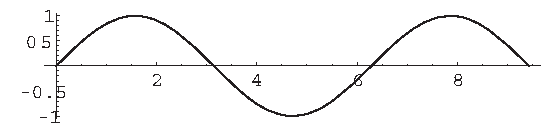
\includegraphics[width=2.5in]{image1.pdf}
  \caption{Caption da figura}
  \label{fig:teste}
\end{figure}


\section{Resultados Esperados}

Descrever quais os resultados que são esperados com a realização dessa pesquisa. 
  
\bibliographystyle{plain} 
\bibliography{ref}
  
\end{document} 
